\documentclass[twocolumn]{article}
\usepackage[utf8]{inputenc}
\usepackage[english]{babel}
\usepackage{hyperref}
\usepackage{lipsum}% http://ctan.org/pkg/lipsum
\usepackage{graphicx}% http://ctan.org/pkg/graphicx
\usepackage{multicol}
\usepackage{natbib}
\setlength{\parindent}{4em}


	\addtolength{\oddsidemargin}{-0.4in}
	\addtolength{\evensidemargin}{-0.4in}
	\addtolength{\textwidth}{0.9in}
	\addtolength{\topmargin}{-1.5in}
	\addtolength{\textheight}{1.3in}

\begin{document}
    \begin{titlepage}
       \begin{center}
            \vspace*{1cm}
            \huge
            \textbf{Higher Education: Course Satisfaction and what influences it}
            
            \large
            \vspace{2cm}
            A school project
     
            \vspace{1.5cm}
            
                Olsen, Lars-Peter \\
                Lützen, Luis Osorio \\ 
                Muntean, Bogdan \\
        
           \vfill
           \vspace{0.8cm}
     
           Data Science\\
           KEA - Copenhagen School of Design and Technology\\
           Denmark\\
           \date{October 2019}
       \end{center}
    \end{titlepage}

% Table of contents %
\begin{titlepage}
    \vspace*{10cm}
    \tableofcontents{}
\end{titlepage}


% Abstract %
\begin{abstract}
The present paper analyses the correlation between course satisfaction as assessed by students and several factors regarding teachers such as helpfulness and commitment, preparation and organization, competence and ethics. The articles argues that CEQs - Course Experience Questionnaires -  are a good way to assess student satisfaction, yet proper questionnaire design is required. Lastly, it emphasizes on the importance of teachers in the context of a higher educational institution and how the course satisfaction rate fluctuates in tandem with teacher’s’ competence and ethics.
\end{abstract}

% Introduction %
\section{Introduction} \label{introduction}

Higher education sits at the very base of our societal development. Whether we are talking about the economic development \cite{Lin2004} or we are exploring different academical research fields \cite{Jones}, it is commonly agreed that higher education nurtures progress, both on an individual level, as well as when it comes to field advancements. In the brink of globalization, cities are competing in different categories; be it wealth, research, talent or investment \cite{Caniels2011}. Certain cities will label themselves as leaders in a field, but it is because of well established educational institutions that specialize in these very fields that such claims can be made \cite{Caniels2011}.

Having said that, it is important to understand that teachers are the most important factor when it comes to determining whether a subject, program or educational institution is efficient and provides results or not \cite{Hattie}. By stating that, we are not neglecting the tools and means that an educational institution can provide, but rather state that without qualified staff that is competent to teach while leveraging such assets, progress is impeded \cite{guyana}.

Altun et al. discovers that teacher commitment to their job does in fact reflect to the students achievements and course satisfaction. He goes as far as proving that teacher commitment is at the core of quality education \cite{Altun2017}. V.Danetta et al. identifies 22 factors that influence teachers commitment to student learning \cite{Dannetta2002} and categorizes them into personal and organizational factors. This theme is further explored by Altun et al. \cite{Altun2017}, proving that a strong correlation between competence and commitment among teachers exists by using the Person Correlation Coefficient \cite{Akram}.

Such claims are supported by various studies that have identified frameworks and methods of assessing the quality of a teacher through the use of questionnaires \cite{Ramsden1991}, \cite{Kember2009}. These explore various themes by which a student is assessing his/her teacher based on their experience. Ramsden et al. shows that Course Experience Questionnaires (CEQ) are a reliable, scalable and useful method of assessing student satisfaction for a course as well as providing feedback to the teacher \cite{Ramsden1991}. If well built, a questionnaire can provide the needed information to objectively assess the subject in question and in doing so supporting the process of optimizing and improving it \cite{Kember2009}.

In this paper we are exploring different aspects of teaching and how course satisfaction is influenced by the very same factors. It addresses the manner in which a satisfaction questionnaire was built in and the division of the questionnaire into themes/sections to better convey the relationship between course satisfaction and the factors that are influencing it.

The paper is built on a combination of desk study and the analysis of a data set which represents the answers of 5820 students to a satisfaction questionnaire that assesses three teachers responsible for thirteen subjects/classes. No other information is known about either the subject/class, the teacher or the  students that in question other than the data set itself. Therefore, assumptions will be made in Section (\ref{analysis}) with the intent of making more sense out of the data.

The rest of the paper will describe the used research methods in Section (\ref{methods}), Section (\ref{analysis}) presents the analysis that was performed on the data while taking into consideration the assumptions that we have made, Section (\ref{findings}) presents the findings of our study and Section (\ref{conclusion}) concludes the paper.

% Methods %
\section{Methods} \label{methods}

This paper implements a mixed-method approach where we are combining desk research with empirical findings. Our empirical findings are based on a satisfaction questionnaire from a higher educational institution where three instructors - that are teaching 13 classes - are assessed with 28 questions graded from 1 to 5 on a likert type scale. This method has proven to be effective, scalable and reliable as Ramsden et al. points out in his study \cite{Ramsden1991}. Therefore, document analysis, enhanced by the exploration of the given data set will be the primary approach to this paper.

In Nunamaker et al. research methods are addressed and argued for \cite{Nunamaker}. The focus is on five primary types of research methods. Out of these five we have identified the \textit{Formulative and Verification Research (Exploratory Research)} as being the best fit for the given scenario. With it, we are trying to identify problems for more precise investigation, raise awareness about the subject at hand and gain insight into the problem area. In short, we are formulating a hypothesis which will either be supported or refuted by our empirical findings \cite{Nunamaker}.

The hypothesis is built on exploring well cited scientific articles \cite{Dannetta2002}, \cite{Altun2017} which correlate course satisfaction and student success with the activity of a teacher in the context of a higher educational institution. Therefore, the activity of the three teachers is assessed with the help of a satisfaction questionnaire where 5820 students have answered to 28 questions. Such activity is encouraged by Kember et al. and was proved useful when optimizing a process and therefore improving it \cite{Kember2009}. The entries are anonymised and little is known about the teacher, course or student other than teacher id, class id, the number of times that a student took that course, the difficulty of the course as assessed by the student and the entries for the 28 questions from the questionnaire.

This analysis explores a couple of recurring motifs - designing a satisfaction questionnaire \cite{Krosnick2010}, assessing and ranking the teachers based on the entries from the questionnaire and exploring the correlation between Course Satisfaction and three themes \cite{Dannetta2002}, \cite{Altun2017}, namely the helpfulness and commitment shown by a teacher, the preparation and organization shown in his/her course and the competence and ethics exerted while teaching the course \cite{Akram}.  

% Analysis %
\section{Analysis} \label{analysis}

Initially, we addressed the data set in question as being ready for analysis. At a closer inspection we performed some preparatory work, in order to enhance the findings and to have a  better understanding of the research question described in Section (\ref{introduction}). Chapter 5, 7, 9 and 10 of the book 'Data preparation and Data Mining' \cite{Pyle1999} specifically addresses this activity, we therefore following it. In the coming sections we will explore some of the assumptions that we have made with regards to the alteration of the data set. As a rule of a thumb, we chose to exclude or not take into consideration data points and facts that are individually assumed. Such cases are the attendance code and even the nb.repeat column as they do not reflect nor contribute to this case study.

    \subsection{Assumptions} 
    
\emph{1. Altering the scale of 1/5 to -2/2} \\
The first step when reworking the data set and preparing it for further analysis was to convert the 1/5 scale to a -2/2 scale. The main reasons for this choice are a) to have 0 as an average answer and therefore nurture better insight on an uneven value and b) to format the data in a more accessible form with the intent to appeal to a wider audience. In retrospective, this decision has helped us immensely when performing descriptive and inferential statistics on the data set.

Initially, we believed that having a likert scale with uneven options will impede our process as individuals tend to choose the middle value when presented with that option. However, Shing-On Leung describes in his research on comparing likert scales of different points that the mean, standard deviation and standard error remain consistent between even and uneven likert scale points, yet the distribution is more consistent on a likert scale that has 11 points \cite{Leung2011}.

\emph{2. Faulty records} \\
By looking at the data, we have observed that there are a plethora of records that have all the values between Q1 and Q28 and even the difficulty the same score. We have decided to eliminate such records on the basis of such records skewing the results when performing analyisis on the data set. Encouraged by Bishop et al. who states that it is important to address likert uneven scales as they have a difficulty in expressing consistency \cite{Bishop}. He goes further to criticize such scales on the basis that though the data itself is easier to collect, it does not provide a statistical power of the likes of Pearson Correlation and other statistical derivatives \cite{Bishop}.

\emph{3. Identifying duplicate questions} \\
At a closer inspection, we have identified a number of questions that seem to repeat throughout the questionnaire. Researching this fact brought us to the conclusion that in more than one cases, questionnaire authors are rephrasing questions with the intent to assess the consistency with which the audience has answered \cite{Rattray2007}, \cite{Krosnick2010}. 

Such questions are Q5 and Q7, Q8 and Q10, Q13 and Q14, Q15 and Q19, Q16 and Q18, Q20 and Q25, Q21 and Q22 as well as Q24 and Q26. We then proceeded to testing this hypothesis by calculating the difference between each pair of questions. If the result was greater than modulus 1, we would mark the question entry as Positive, otherwise Negative. 
The number of Positive entries did not exceed 5\% of the dataset before we have eliminated the records which we considered faulty and was less than 10\% after the exclusion was made.

\begin{center}
\centering
 \begin{tabular}{ |c| c| c| }
    \hline
     Pair & Positive values\\ 
     \hline
     Q5 and Q7 & 255\\  
     \hline
     Q8 and Q10& 243\\  
      \hline
     Q13 and Q14 & 97\\  
      \hline
     Q15 and Q19 & 238\\  
      \hline
     Q16 and Q18 & 187\\  
      \hline
     Q20 and Q25 & 223\\  
      \hline
     Q21 and Q22 & 101\\  
      \hline
     Q24 and Q16 & 281\\  
     \hline
    \end{tabular} \\
\caption{Positive values per pair of questions after the faulty entries have been eliminated}
  \label{table:1}
\end{center}
With this in mind, our hypothesis was proven right, and the next step was to condense the pairs of questions into one column per pair - by calculating the mean per entry for the pair of questions. We have done that to create a more condensed version of the data set.

\emph{4. The questionnaire is divided into themes} \\
With the help of Krosnik et al. \cite{Krosnick2010} and Kember et al \cite{Kember2009} we understood that usually, with likert scale questionnaires, there are a handfull of themes that are addressed and each theme is divided into a number of questions. When the analysis is performed, the answers to these questions are condensed back into the original themes and an easier, more robust process can be applied on the data to gain insight in it. \cite{Kember2009}

Our assumption was that there are four themes that are consistently showing up in the questionnaire. After much debate, we have grouped the 20 remaining questions into four themes, five questions per theme.

\begin{center}
\centering
 \begin{tabular}{ |c| c| c| }
    \hline
     Code & Theme & Questions\\ 
     \hline
     C.S. & Course Satisfaction & \makecel{3,5-7,9,11,8-10}\\  
     \hline
     P.O. & Prep./Org. & 1,2,4,15-19,24-26\\  
      \hline
     C.E & Competence/Ethics &6,13-14,16-18,17,28\\  
      \hline
     H.C. & Help/Commit &12,27,23,21-22,20-25\\  
      \hline
    \end{tabular} \\
\caption{The questions that will be grouped together based on the identified theme}
  \label{table:2}
\end{center}

\emph{5. Individually assumed facts} \\

We are calling an individually assumed fact a hypothesis that only has one piece of evidence and no more than one datapoint to relate to, which in our case is itself. Pursuing our ethical commitment towards this academic paper, we are choosing to ignore the attendance column on the basis that it cannot be related to another column or datapoint and gain solid insights from it.

As far as the nb.repeats column, we did believe that there is a relationship between it and the questions from the questionnaire. That is not the case however as further analysis has shown and by utilizing the Pearson Coefficient. Alas, we are ignoring this column as well.

    \subsection{CEQ - usage}
Ramsden et al. states that higher education has its focus on research outputs rather than the teaching functions of educational institutions \cite{Ramsden1991}. He proposes a model meant to evaluate teachers with the help of a CEQ - Course experience questionnaire. The provided data set carries a similar function and therefore will be looked at as an instrument of measurement for performance. 

\begin{figure}[hbt!]
  \centering
  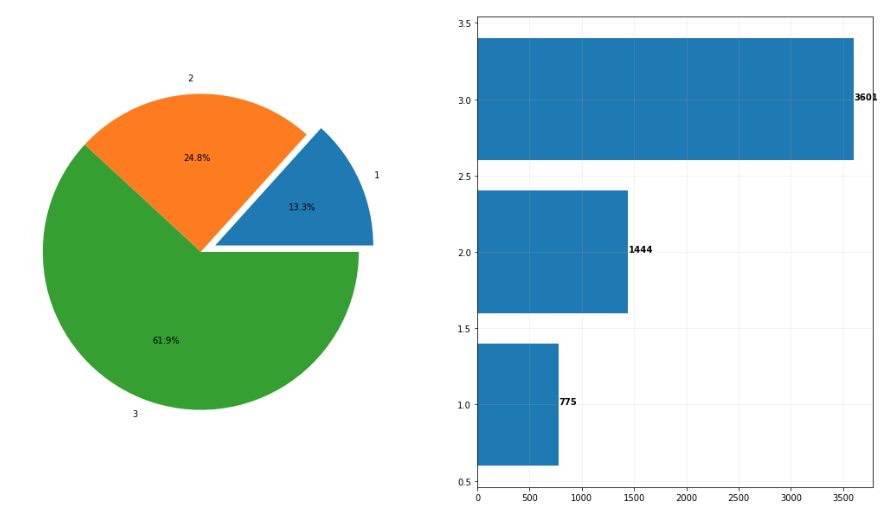
\includegraphics[width=3.5in]{teach_dist.png}
  \caption{The student distribution per teacher}
\end{figure}

Lastly, such questionnaire can be used in order to provide feedback to each teacher, anonymously and hopefully truthfully. Therefore, based on the circumstances under which a teacher is in, the teacher can assess whether an improvement can be done in his/her teaching career so that the students can benefit out of such questionnaires \cite{Kember2009}.

    \subsection{Course Satisfaction}

A great part of this analysis was spent on correlating the data set and identifying the factors that drive teacher commitment and student satisfaction towards the course itself. Danetta et al. identifies 22 factors that contribute to student learning \cite{Dannetta2002}. He then further divides them into organizational factors and personal factors. As is now, there is no information regarding the organization itself in the data set. However we can make use of the great majority of the factors presented by Danetta et al. as they refer to how student learning and course satisfaction is influenced by the teachers commitment \cite{Dannetta2002}. 

Altun et al. is proving that there is a strong correlation between competence and commitment among teachers, result that he found by applying the Pearson Correlation Coefficient \cite{Altun2017}. This realization ties into the original hypothesis from Section (\ref{introduction}) where we claim that course satisfaction is influenced by certain factors and as we later on explain these factors are teacher commitment, competence and preparation. 

    \subsection{Pearson Correlation Coefficient}

The Pearson correlation is used to quantify the degree of colocalization between different data points. Adler et al. is proving that the pearson correlation is superior to the Mander's overlap coefficient \cite{Adler2010}. While the two are really similar, they differ in the use of either the absolute intensities (MOC) and the deviation from the mean (PCC), hence we are making use of it to understand if there is a correlation between the aforementioned themes.

By applying ourselves the Pearson Correlation Coefficient on the dataset, we are noticing that there is a strong correlation between the course satisfaction, the commitment of a teacher and his competence.

    \begin{figure}[hbt!]
      \centering
      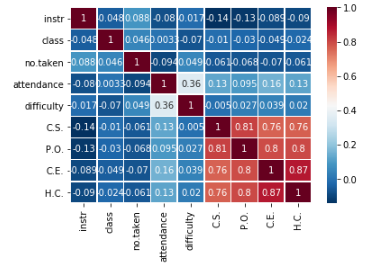
\includegraphics[width=3.5in]{pcds.png}
      \caption{PCC applied on the whole dataset}
      \label{fig:2}
    \end{figure}

In Figure: \ref{fig:2} an overal correlation can be observed between the mentioned themes. Section (\ref{findings}) will explore this in more detail.

    \subsection{Ranking the teachers}
 
 Moreover,  a ranking of the three students will be provided keeping in mind that circumstances are different for each teacher - one teacher is teaching three classes, another teaches four and the last one teaches seven classes and the classes that they are teaching are of various sizes.
 
 Nevertheless, from the performed analysis, we wanted to assess whether the teachers are consistent - which they are - and if the scores have anything to do with the amount of courses and students that they are teaching - which it does.
 
 In Figure: \ref{fig3} the ranks of teachers based on the four categories: Course Satisfaction, Competence and Ethics, Helpfulness and Commitment and Preparation and Organization can be observed.
   
\begin{figure}
  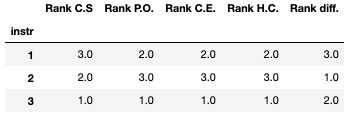
\includegraphics[width=0.5\textwidth,height=4cm]{r.png}
  \caption{Teacher ranks overall}
  \label{fig3}
\end{figure}

% Findings %
\section{Findings} \label{findings}
Based on our analysis and by using Pearson's Correlation Coefficient, we have established that there is indeed a strong relationship between the course satisfaction as assessed by the students and the other outlined themes. 

Ranking the correlations, we can observe that teachers that have a higher score in the competence and ethics theme are overall more helpful towards the students. Based on that and our desk research where we identified the benefits of teacher's commitment towards improving learning and course satisfaction, it is advised to improve the competence of the teachers so as to maximize the course satisfaction and student achievements.

Secondary to that, the more prepared a teacher is for his/her course, the better course satisfaction students will experience.

\begin{figure}
  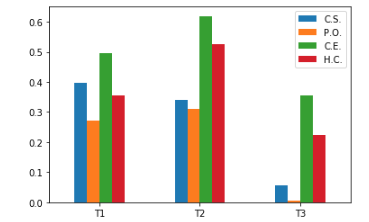
\includegraphics[width=0.5\textwidth,height=4cm]{tt.png}
  \caption{Teacher scores side by side in all the 4 explored themes}
  \label{fig4}
\end{figure}

Nevertheless, there is a small correlation between the difficulty of the course as perceived by the students and the attendance column, however, without knowing what the code stands for, we choose not to interpret this finding.

Lastly, we have identified a clear relationship between the number of courses an instructor teaches and his/her competence as assessed by the students, which is normal. Additionally, we believe that course satisfaction is influenced by the course difficulty.

What we failed to assess is to answer the original research question which was: Is a teacher good or not. We were not able to assess if that is the case as there are simply to few datapoints to relate and there is no way that we can assess what is the absolute good teacher or the absolute bad teacher, hence refrained from pursuing such an analysis.

% Conclusion %
\section{Conclusion} \label{conclusion}
This paper represents a mixed method research that is exploring the correlations between course satisfaction and teacher commitment, competence and organization. Based on Danetta et al. \cite{Dannetta2002} and Altun et al. \cite{Altun2017}- with the help of which we have formulated our research question - and supported by our empirical findings, the correlation between the course satisfaction as assessed by the students and teacher commitment, competence and preparation.

We have identified however areas that this research does not cover namely, a more in depth analysis of the teacher’s activity per class as well as the probability of more correlations being present in the given dataset.

We therefore conclude that CEQ is a feasible method to gain feedback and plan on future teacher improvements, yet we are advising towards formulating the questionnaire with certain factors in mind, primarily what scale is to be used and limiting it to a handful of themes so as to ensure consistency.

The Jupyter Notebook can be found here:  \url{https://github.com/bgz10/DS_MA_Q.git} 

% References %
\bibliographystyle{plain}
\bibliography{references.bib}
\end{document}
